\documentclass[11pt,a4paper]{article}
\usepackage[margin=1in, headheight=14pt]{geometry}
\usepackage{amsfonts,amsmath,amssymb,suetterl}
\usepackage{lmodern}
\usepackage[T1]{fontenc}
\usepackage{fancyhdr}
\usepackage{float}
\usepackage[utf8]{inputenc}
\usepackage{fontawesome}
\usepackage{enumerate}
\usepackage{xcolor}
\usepackage{hyperref}
\usepackage{tikz}
\usepackage{nicefrac}
\usepackage{subcaption}
\usepackage{physics}
\usepackage{mathtools}
\usepackage{adjustbox}

\DeclareUnicodeCharacter{2212}{-}

\usepackage{mathrsfs}
\usepackage[nodisplayskipstretch]{setspace}

\setstretch{1.5}
\renewcommand{\footrulewidth}{0pt}

\pagestyle{fancy}
\fancyhead[R]{Problem Sheet 4 (Solutions)}
\fancyhead[L]{MA202: Differential Equations}

\parindent 0ex
\setlength{\parskip}{1em}
\raggedbottom

\begin{document}
	\begin{center}
		\textbf{Problem Sheet 4 - Solutions}
	\end{center}
	%
	\begin{enumerate}
		\item \textbf{(A)} The characteristic equation is given by
		$$
		\begin{vmatrix}
			1-r & -i\\
			i & 1-r
		\end{vmatrix} = (1-r)^2 + i^2 = r(r - 2) = 0.
		$$
		The equation has roots $r_1 = 0$ and $r_2 = 2$. For $r = 0$, the components of the solution vector must satisfy $\xi_1 − i\xi_2 = 0$. Thus the corresponding eigenvector is $\xi^{(1)} = (1, -i)^T$. Substitution of $r = 2$ results in the single equation $-\xi_1 - i\xi_2 = 0$. A corresponding eigenvector is $\xi^{(2)} = (1, i)^T$. Since the eigenvalues are distinct, the general solution is
		$$
		\xi(t) = c_1
		\begin{pmatrix}
			1\\
			-i
		\end{pmatrix} + c_2
		\begin{pmatrix}
			1\\
			i
		\end{pmatrix}e^{2t}.
		$$
		\textbf{(B)} The characteristic equation is given by
		$$
		\begin{vmatrix}
			2-r & 2+r\\
			-1 & -1-i-r
		\end{vmatrix} = r^2 -(1-i)r-i=0.
		$$
		The equation has complex roots $r_1 = 1$ and $r_2 = -i$. For $r = 1$, the components of the solution vector must satisfy $\xi_1 + (2 + i)\xi_2 = 0$. Thus the corresponding eigenvector is $\xi^{(1)} = (2 + i, −1)^T$. Substitution of $r = -i$ results in the single equation $\xi_1 + \xi_2 = 0$. A corresponding eigenvector is $\xi^{(2)} = (1, −1)^T$. Since the eigenvalues are distinct, the general solution is
		$$
		\vb{x}(t) = c_1
		\begin{pmatrix}
			2+i\\
			-1
		\end{pmatrix}e^t + c_2
		\begin{pmatrix}
			1\\
			-1
		\end{pmatrix}e^{-it}.
		$$
		\textbf{(C)} Setting $\vb{x} = \xi e^{rt}$ results in the algebraic equations
		$$
		\begin{pmatrix}
			1-r & 1 & 2\\
			1 & 2-r & 1\\
			2 & 1 & 1-r
		\end{pmatrix}
		\begin{pmatrix}
			\xi_1\\
			\xi_2\\
			\xi_3
		\end{pmatrix} =
		\begin{pmatrix}
			0\\
			0\\
			0
		\end{pmatrix}.
		$$
		For a nonzero solution, we must have $\det(\vb{A} - r\vb{I}) = r^3 - 4r^2 - r + 4 = 0$. The roots of the characteristic equation are $r_1 = 4,\ r_2 = 1$ and $r_3 = −1$. Setting $r = 4$, we have
		$$
		\begin{pmatrix}
			-3 & 1 & 2\\
			1 & -2 & 1\\
			2 & 1 & -3
		\end{pmatrix}
		\begin{pmatrix}
			\xi_1\\
			\xi_2\\
			\xi_3
		\end{pmatrix}=
		\begin{pmatrix}
			0\\
			0\\
			0
		\end{pmatrix}.
		$$
		This system is reduces to the equations
		\begin{align*}
			\xi_1 - \xi_3 &= 0,\\
			\xi_2 - \xi_3 &= 0.
		\end{align*}
		A corresponding solution vector is given by $\xi^{(1)} = (1, 1, 1)^T$. Setting $r = 1$, the reduced system of equations is
		\begin{align*}
			\xi_1 - \xi_3 &= 0,\\
			\xi_2 + 2\xi_3 &= 0.
		\end{align*}
		A corresponding solution vector is given by $\xi^{(2)} = (1, −2, 1)^T$. Finally, setting $r = -1$, the reduced system of equations is
		\begin{align*}
			\xi_1 + \xi_3 &= 0,\\
			\xi_2 &= 0.
		\end{align*}
		A corresponding solution vector is given by $\xi^{(3)} = (1, 0, −1)^T$. Since the eigenvalues are distinct, the general solution is
		$$
		\vb{x}(t) = c_1
		\begin{pmatrix}
			1\\
			1\\
			1
		\end{pmatrix}e^{4t} + c_2
		\begin{pmatrix}
			1\\
			-2\\
			1
		\end{pmatrix}e^t + c_2
		\begin{pmatrix}
			1\\
			0\\
			-1
		\end{pmatrix}e^{-t}.
		$$
		\item \textbf{(A)} Setting $\vb{x} = \xi e^{rt}$ results in the algebraic equations
		$$
		\begin{pmatrix}
			3-r & 4\\
			-2 & -1-r
		\end{pmatrix}
		\begin{pmatrix}
			\xi_1\\
			\xi_2
		\end{pmatrix}=
		\begin{pmatrix}
			0\\
			0
		\end{pmatrix}.
		$$
		For a nonzero solution, we require that $\det(\vb{A} - r\vb{I}) = r^2 - 2r + 5 = 0$. The roots of the characteristic equation are $r_{1,2} = 1 \pm 2i$. Substituting $r = 1 - 2i$, the two equations reduce to
		$$
		(1+i)\xi_1 + 2\xi_2 = 0.
		$$
		The eigenvector is $\xi^{(1)} = (2, -1 - i)^T$. Hence one of the complex-valued solutions is given by
		\begin{align*}
			\displaybreak
			\vb{x}^{(1)} &=
			\begin{pmatrix}
				2\\
				-1-i
			\end{pmatrix}e^{(1-2i)t} =
			\begin{pmatrix}
				2\\
				-1-i
			\end{pmatrix}e^t(\cos 2t + i\sin 2t)\\
			&= e^t
			\begin{pmatrix}
				2\cos 2t\\
				-\cos 2t - \sin 2t
			\end{pmatrix} + ie^t
			\begin{pmatrix}
				-2\sin 2t\\
				\sin 2t - \cos 2t
			\end{pmatrix}.
		\end{align*}
		To find real-valued solutions, we take the real and imaginary parts, respectively, of $\vb{x}^{(1)}(t)$:
		$$
		\vb{x} = c_1e^t
		\begin{pmatrix}
			2\cos 2t\\
			-\cos 2t - \sin 2t
		\end{pmatrix} + c_2e^t
		\begin{pmatrix}
			-2\sin 2t\\
			\sin 2t -\cos 2t
		\end{pmatrix}.
		$$
		\textbf{(B)} Solution of the ODEs is based on the analysis of the algebraic equations
		$$
		\begin{pmatrix}
			2-r & 1\\
			-5 & -2-r
		\end{pmatrix}
		\begin{pmatrix}
			\xi_1\\
			\xi_2
		\end{pmatrix} = 
		\begin{pmatrix}
			0\\
			0
		\end{pmatrix}.
		$$
		For a nonzero solution, we require that $\det(\vb{A} - r\vb{I}) = r^2 + 1 = 0$. The roots of the characteristic equation are $r_{1,2} = \pm i$. Setting $r = i$, the equations are equivalent to $(2 - i)\xi_1 + \xi_2 = 0$. The eigenvectors are $\xi^{(1)} = (1, -2 + i)^T$ and $\xi^{(1)} = (1, -2 - i)T$. Hence one of the complex-valued solutions is given by
		\begin{align*}
			\vb{x}^{(1)}(t) &=
			\begin{pmatrix}
				1\\
				-2+i
			\end{pmatrix}e^{it} =
			\begin{pmatrix}
				1\\
				-2+i
			\end{pmatrix}(\cos t + i\sin t)\\
			&=
			\begin{pmatrix}
				\cos t\\
				-2\cos t - \sin t
			\end{pmatrix} + i
			\begin{pmatrix}
				\sin t\\
				\cos t - 2\sin t
			\end{pmatrix}.
		\end{align*}
		%
		\begin{figure}[H]
			\centering
			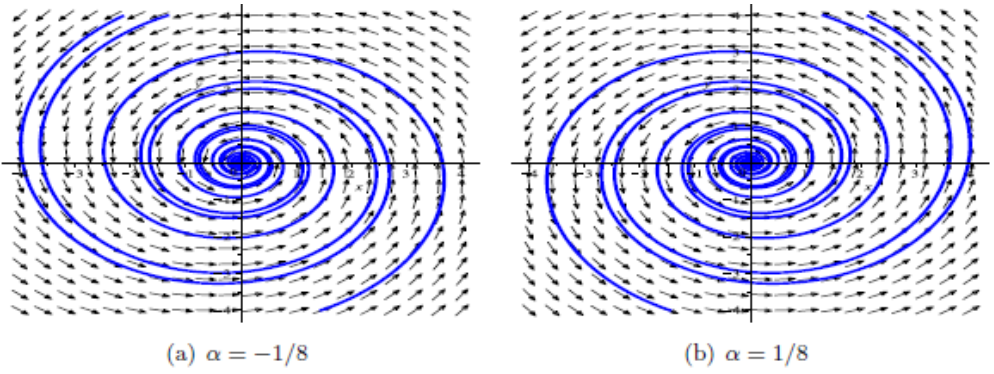
\includegraphics[width=0.75\textwidth]{figure/4_fig1.PNG}
			\caption{The phase portrait for the system in Question 5A.}
		\end{figure}
		%
		Therefore the general solution is
		$$
		\vb{x}(t) = c_1
		\begin{pmatrix}
			\cos t\\
			-2\cos t - \sin t
		\end{pmatrix} + c_2
		\begin{pmatrix}
			\sin t\\
			\cos t -2\sin t
		\end{pmatrix}.
		$$
		The solution may also be written as
		$$
		\vb{x(t)} = c_1
		\begin{pmatrix}
			-2\cos t + \sin t\\
			5\cos t
		\end{pmatrix} + c_2
		\begin{pmatrix}
			-2\sin t - \cos t\\
			5\sin t
		\end{pmatrix}
		$$
		\item \textbf{(A)} The characteristic equation is $r^2 - 2\alpha r + 1 + \alpha^2 = 0$, with roots $r = \alpha \pm i$. (b) When $\alpha < 0$ and $\alpha > 0$, the equilibrium point $(0, 0)$ is a stable spiral and an unstable spiral, respectively.\\
		The equilibrium point is a center when $\alpha = 0$. The phase portraits for different values of $\alpha$ are shown in Fig. 1.\\
		\textbf{(B)} The roots of the characteristic equation, $r^2 - \alpha r + 5 = 0$, are
		$$
		r_{1,2} = \frac{\alpha}{1}\pm \frac{1}{2}\sqrt{\alpha^2 - 20}.
		$$
		Note that the roots are complex when $- \sqrt{20} < \alpha < \sqrt{2}$. For the case when $\alpha \in (-\sqrt{20}, 0)$, the equilibrium point $(0, 0)$ is a stable spiral. On the other hand, when $\alpha \in (0, \sqrt{20})$, the equilibrium point is an unstable spiral.\\
		For the case $\alpha = 0$, the roots are purely imaginary, so the equilibrium point is a center.\\
		When $\alpha^2 > 20$, the roots are real and distinct. The equilibrium point becomes a node, with its stability dependent on the sign of $\alpha$. Finally, the case $\alpha^2 = 20$ marks the transition from spirals to nodes (see Fig. 2).
		\item Setting $\vb{x} = \xi e^{rt}$, and substituting into the ODE, we obtain the algebraic equations
		$$
		\begin{pmatrix}
			3-r & 2\\
			-2 & -2-r
		\end{pmatrix}
		\begin{pmatrix}
			\xi_1\\
			\xi_2
		\end{pmatrix} =
		\begin{pmatrix}
			0\\
			0
		\end{pmatrix}.
		$$
		For a nonzero solution, we require that $\det(\vb{A} - r\vb{I}) = r^2 - r - 2 = 0$. The roots of the characteristic equation are $r_1 = -1$ and $r_2 = 2$. For $r = -1$, the two equations reduce
		%
		\begin{figure}[H]
			\centering
			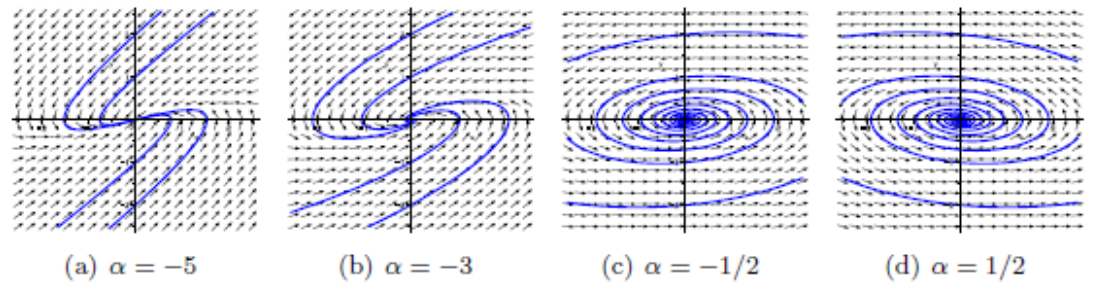
\includegraphics[width=0.85\textwidth]{figure/4_fig2.PNG}
			\caption{The phase portrait for the system in Question 5B.}
		\end{figure}
		%
		to $2\xi_1 = -\xi_2$. The corresponding eigenvector is $\xi^{(1)} = (−1, 2)^T$. Substitution of $r = 2$ results in the single equation $\xi_1 = -2\xi_2$. A corresponding eigenvector is $\xi^{(2)} = (-2, 1)^T$. The general solution is
		$$
		\vb{x}(t) = c_1
		\begin{pmatrix}
			-e^{-t}\\
			2e^{-t}
		\end{pmatrix} + c_2
		\begin{pmatrix}
			-2e^{2t}\\
			e^{2t}
		\end{pmatrix}.
		$$
		Hence a fundamental matrix is given by
		$$
		\Psi (t) =
		\begin{pmatrix}
			-e^{-t} & -2e^{2t}\\
			2e^{-t} & e^{2t}
		\end{pmatrix},
		$$
		Then we have
		$$
		\Psi(0) =
		\begin{pmatrix}
			-1 & -2\\
			2 & 1
		\end{pmatrix},\qquad \Psi^{-1}(0) = \frac{1}{3}
		\begin{pmatrix}
			1 & 2\\
			-2 & -1
		\end{pmatrix}.
		$$
		So that
		$$
		\Phi(t) = \Psi(t)\Psi^{-1}(0) = \frac{1}{3}
		\begin{pmatrix}
			-e^{-t} + 4e^{2t} & -2e^{-t} + 2e^{2t}\\
			2e^{-t}-2e^{2t} & 4e^{-t} - e^{2t}
		\end{pmatrix}.
		$$
		\textbf{(B)} The characteristic equation reduces to $r^2 + r - 6 = 0$. The roots of the characteristic equation are $r_1 = 2$ and $r_2 = -3$. For $r = 2$, the system of equations reduces to $\xi_1 = 4\xi_2$. The corresponding eigenvector is $\xi^{(1)} = (4, 1)^T$. Substitution of $r = -3$ results in the single equation $\xi_1 + \xi_2 = 0$. A corresponding eigenvector is $\xi^{(2)} = (1, -1)^T$. Hence, we have the two linearly independent solutions
		$$
		\vb{x}^{(1)} =
		\begin{pmatrix}
			4\\
			1
		\end{pmatrix}e^{2t},\qquad \vb{x}^{(1)} =
		\begin{pmatrix}
			1\\
			-1
		\end{pmatrix}e^{-3t}.
		$$
		Thus
		$$
		\Psi(t) =
		\begin{pmatrix}
			4e^{2t} & -e^{-3t}\\
			e^{2t} & e^{-3t}
		\end{pmatrix}.
		$$
		Imposing the canonical initial condition we get
		$$
		\Psi(0) =
		\begin{pmatrix}
			4 & -1\\
			1 & 1
		\end{pmatrix},\quad \text{and} \quad \Psi^{-1}(0) =
		\begin{pmatrix}
			1 & 1\\
			-1 & 4
		\end{pmatrix},
		$$
		so that
		$$
		\Phi(t) = \Psi(t)\Psi^{-1}(0) = \frac{1}{5}
		\begin{pmatrix}
			e^{-3t} + 4e^{2t} & -4e^{-3t} + 4e^{2t}\\
			-e^{-3t} + e^{2t} & 4e^{-3t} + e^{2t}
		\end{pmatrix}.
		$$
		\item \textbf{(A)} Assuming that $\vb{x} = \phi(t)$ is a solution, then $\phi^\prime = \vb{A}\phi$, with $\phi(0) = \vb{x}^0$. Integrate both sides of the equation to obtain
		$$
		\phi(t) - \phi(0) = \int_0^t \vb{A}\phi(s)ds.
		$$
		Hence
		$$
		\phi(t) = \vb{x}^0 + \int_0^t \vb{A}\phi(s)ds.
		$$
		\textbf{(B)} Proceed with the iteration
		$$
		\phi(t)^{(i+1)} = \vb{x}^0 + \int_0^t \vb{A}\phi^{(i)}(s)ds.
		$$
		With $\phi^{(0)}(t) = \vb{x}^0$, and noting that $\vb{A}$ is a constant matrix,
		$$
		\phi^{(1)}(t) = \vb{x}^0 + \int_0^t \vb{A}\vb{x}^0ds = \vb{x}^0 + \vb{A}\vb{x}^0t.
		$$
		That is, $\phi^{(1)}(t) = (\vb{I} + \vb{A}t)\vb{x}^0$.\\
		\textbf{(C)} We then have
		$$
		\phi^{(2)}(t) = \vb{x}^0 + \int_0^t \vb{A}(\vb{I} + \vb{A}t)\vb{x}^0ds = \vb{x}^0 + \vb{A}\vb{x}^0 t + \vb{A}^2\vb{x}^0\frac{t^2}{2} = \left(\vb{I} + \vb{A}t + \vb{A}^2 \frac{t^2}{2}\right)\vb{x}^0.
		$$
		Now suppose that
		$$
		\phi^{(n)}(t) = \left(\vb{I} + \vb{A}t + \vb{A}\frac{t^2}{2} + \ldots + \vb{A}\frac{t^n}{n!}\right)\vb{x}^0.
		$$
		It follows that
		\begin{align*}
			& \int_0^t \vb{A}\left(\vb{I} + \vb{A}t + \vb{A}^2\frac{t^2}{2} + \ldots + \vb{A}^n\frac{t^n}{n!}\right)\vb{x}^0ds\\
			&= \vb{A}\left(\vb{I}t + \vb{A}^2\frac{t^2}{2} + \vb{A}^2\frac{t^3}{3!} + \ldots + \vb{A}^n\frac{t^{n+1}}{(n+1)!}\right)\vb{x}^0\\
			&= \left(\vb{A}t + \vb{A}\frac{t^2}{2} + \vb{A}^3\frac{t^3}{3!} + \ldots + \vb{A}^{n+1}\frac{t^{n}}{n!}\right)\vb{x}^0.
		\end{align*}
		Therefore
		$$
		\phi^{(n+1)}(t) = \left(\vb{I}t + \vb{A}\frac{t^2}{2} + \vb{A}^2\frac{t^3}{3!} + \ldots + \vb{A}^{n+1}\frac{t^{n+1}}{(n+1)!}\right)\vb{x}^0.
		$$
		By induction, the asserted form of $\phi^{(n)}(t)$ is valid for all $n \geq 0$.\\
		\textbf{(D)} Define $\phi^{(\infty)}(t) = \lim_{n \ to \infty}\phi^{(n)}(t)$. It can be shown that the limit does exist. In fact,
		$$
		\phi^{(\infty)}(t) = e^{\vb{A}t}\vb{x}^0.
		$$
		Term-by-term differentiation results in
		\begin{align*}
			\frac{d}{dt}\phi^{(\infty)}(t)
			&= \frac{d}{dt}\left(\vb{I} + \vb{A}t + \vb{A}^2\frac{t^2}{2} + \ldots + \vb{A}^n\frac{t^n}{n!} + \ldots\right)\vb{x}^0\\
			&= \left(\vb{A} + \vb{A}^2t + \ldots + \vb{A}^n\frac{t^{n-1}}{(n-1)!} + \ldots\right)\vb{x}^0\\
			&= \vb{A}\left(\vb{I} + \vb{A}t + \vb{A}^2\frac{t^2}{2} + \ldots + \vb{A}^{n-1}\frac{t^{n-1}}{(n-1)!} + \ldots\right)\vb{x}^0.
		\end{align*}
		That is,
		$$
		\frac{d}{dt}\phi^{(\infty)}(t) = \vb{A}\phi^{(\infty)}(t).
		$$
		Furthermore, $\phi^{(\infty)}(0) = \vb{x}^0$. Based on uniqueness of solutions, $\phi(t) = \phi^{(\infty)}(t)$.
		\item \textbf{(A)} Solution of the ODE requires analysis of the algebraic equations
		$$
		\begin{pmatrix}
			1-r & -4\\
			4 & -7-r
		\end{pmatrix}
		\begin{pmatrix}
			\xi_1\\
			\xi_2
		\end{pmatrix} =
		\begin{pmatrix}
			0\\
			0
		\end{pmatrix}.
		$$
		For a nonzero solution, we must have $\det(\vb{A} - r\vb{I}) = r^2 + 6r + 9 = 0$. The only root is $r = −3$, which is an eigenvalue of multiplicity two. Substituting $r = −3$ into the coefficient matrix, the system reduces to the single equation $\xi_1 - \xi_2 = 0$. Hence the corresponding eigenvector is $\xi = (1, 1)^T$. One solution is
		$$
		\vb{x}^{(1)} =
		\begin{pmatrix}
			1\\
			1
		\end{pmatrix}e^{-3t}
		$$
		For a second linearly independent solution, we search for a generalized eigenvector. Its components satisfy
		$$
		\begin{pmatrix}
			4 & -4\\
			4 & -4
		\end{pmatrix}
		\begin{pmatrix}
			\eta_1\\
			\eta_2
		\end{pmatrix} =
		\begin{pmatrix}
			1\\
			1
		\end{pmatrix}.
		$$
		that is, $4\eta_1 - 4\eta_2 = 1$. Let $\eta_2 = k$, some arbitrary constant. Then $\eta_1 = k + 1/4$. It follows that a second solution is given by
		$$
		\vb{x}^{(2)} =
		\begin{pmatrix}
			1\\
			1
		\end{pmatrix}te^{-3t} +
		\begin{pmatrix}
			k+1/4\\
			k
		\end{pmatrix}e^{-3t} =
		\begin{pmatrix}
			1\\
			1
		\end{pmatrix}te^{-3t} +
		\begin{pmatrix}
			1/4\\
			0
		\end{pmatrix}e^{-3t} + k
		\begin{pmatrix}
			1\\
			1
		\end{pmatrix}e^{-3t}.
		$$
		Dropping the last term, the general solution is
		$$
		\vb{x} = c_1
		\begin{pmatrix}
			1\\
			1
		\end{pmatrix}e^{-3t} + c_2
		\left[
			\begin{pmatrix}
				1\\
				1
			\end{pmatrix}te^{-3t} +
			\begin{pmatrix}
				1/4\\
				0
			\end{pmatrix}e^{-3t}
		\right].
		$$
		Imposing the initial conditions, we require that $c_1 + c_2/4 = 4,\ c_1 = 2$, which results in $c_1 = 2$ and $c_2 = 8$. Therefore the solution of the IVP is
		$$
		\vb{x} =
		\begin{pmatrix}
			4\\
			2
		\end{pmatrix}e^{-3t} +
		\begin{pmatrix}
			8\\
			8
		\end{pmatrix}te^{-3t}.
		$$
		The phase plot of the solutions is presented on Figure 3.\\
		\textbf{(B)} The eigensystem is obtained from analysis of the equation
		$$
		\begin{pmatrix}
			3 - r & -1\\
			9 & -3 - r
		\end{pmatrix}
		\begin{pmatrix}
			\xi_1\\
			\xi_2
		\end{pmatrix} =
		\begin{pmatrix}
			0\\
			0
		\end{pmatrix}.
		$$
		The characteristic equation is $r^2 = 0$, with a single root $r = 0$. Setting $r = 0$, the two equations reduce to $3\xi_1 - \xi_2 = 0$. The corresponding eigenvector is $\xi = (1, 3)^T$. Hence one solution is
		$$
		\vb{x}^{(1)} =
		\begin{pmatrix}
			1\\
			3
		\end{pmatrix},
		$$
		%
		\begin{figure}[H]
			\centering
			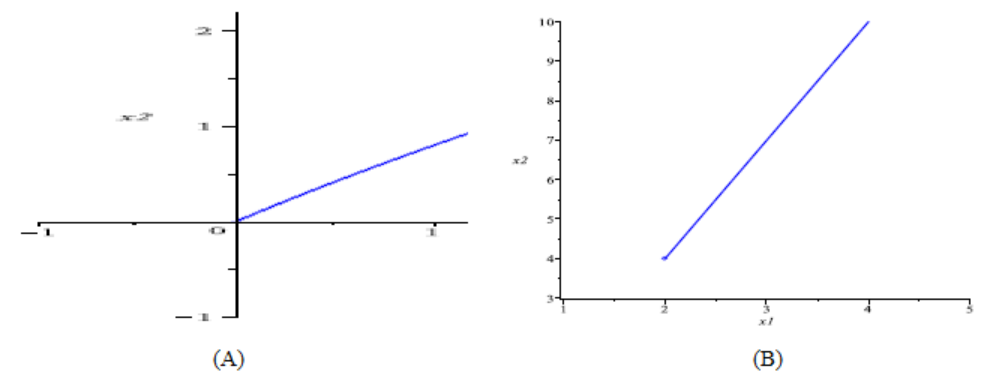
\includegraphics[width=0.85\textwidth]{figure/4_fig3.PNG}
			\caption{The phase of the solutions of the systems in Question 8.}
		\end{figure}
		%
		which is a constant vector. A second linearly independent solution is obtained from the system
		$$
		\begin{pmatrix}
			3 & -1\\
			9 & -3
		\end{pmatrix}
		\begin{pmatrix}
			\eta_1\\
			\eta_2
		\end{pmatrix} = 
		\begin{pmatrix}
			1\\
			3
		\end{pmatrix}.
		$$
		The equations reduce to the single equation $3\eta_1 - \eta_2 = 1$. Let $\eta_1 = k$. We obtain $\eta_2 = -1 + 3k$, and a second linearly independent solution is
		$$
		\vb{x}^{(2)} =
		\begin{pmatrix}
			1\\
			3
		\end{pmatrix}t +
		\begin{pmatrix}
			k\\
			-1+3k
		\end{pmatrix} =
		\begin{pmatrix}
			1\\
			3
		\end{pmatrix}t +
		\begin{pmatrix}
			0\\
			-1
		\end{pmatrix} + k
		\begin{pmatrix}
			1\\
			3
		\end{pmatrix}.
		$$
		Dropping the last term, the general solution is
		$$
		\vb{x}(t) = c_1
		\begin{pmatrix}
			1\\
			3
		\end{pmatrix} + c_2
		\left[
			\begin{pmatrix}
				1\\
				3
			\end{pmatrix}t +
			\begin{pmatrix}
				0\\
				-1
			\end{pmatrix}
		\right].
		$$
		Imposing the initial conditions, we require that $c_1 = 2,\ 3c_1 - c_2 = 4$, which results in $c_1 = 2$ and $c_2 = 2$. Therefore the solution of the IVP is
		$$
		\vb{x}(t) = c_1
		\begin{pmatrix}
			2\\
			4
		\end{pmatrix} + 2
		\begin{pmatrix}
			1\\
			3
		\end{pmatrix}t.
		$$
		\item \textbf{(A)} The eigenvalues of
		$$
		\begin{pmatrix}
			2 & 3\\
			-1 & -2
		\end{pmatrix}
		$$
		are given by $r_1 = 1$ and $r_2 = -1$. The corresponding eigenvectors are given by
		$$
		\xi^{(1)} = 
		\begin{pmatrix}
			-3\\
			1
		\end{pmatrix},\qquad \xi^{(2)} =
		\begin{pmatrix}
			-1\\
			1
		\end{pmatrix}.
		$$
		Therefore, two linearly independent solutions are given by
		$$
		\vb{x}^{(1)} = 
		\begin{pmatrix}
			-3\\
			1
		\end{pmatrix}e^t,\qquad \vb{x}^{(2)} =
		\begin{pmatrix}
			-1\\
			1
		\end{pmatrix}e^{-t}.
		$$
		and
		$$
		\Psi(t) =
		\begin{pmatrix}
			-3e^t & -e^{-t}\\
			e^t & e^{-t}
		\end{pmatrix}
		$$
		is a fundamental matrix. In order to find the general solution using variation of parameters, we need to calculate $\int_{t_1}^t \Psi^{-1}(s)\vb{g}(s)ds$. We see that
		$$
		\Psi^{-1}(s) = \frac{1}{2}
		\begin{pmatrix}
			-e^{-s} & -e^{-s}\\
			e^s & 3e^s
		\end{pmatrix}
		$$
		Therefore,
		\begin{align*}
			\int_{t_1}^t \Psi^{-1}(s)\vb{g}(s)ds
			&= \frac{1}{2}\int_{t_1}^t
			\begin{pmatrix}
				-e^{-s} & -e^{-s}\\
				e^s & 3e^s
			\end{pmatrix}
			\begin{pmatrix}
				e^s\\
				s
			\end{pmatrix}ds\\
			&= \frac{1}{2}\int_{t_1}^t
			\begin{pmatrix}
				-1 - se^{-s}\\
				e^{2s} + 3se^s
			\end{pmatrix}ds = \frac{1}{2}
			\begin{pmatrix}
				-t + te^{-t} + e^{-t}\\
				\frac{1}{2}e^{2t} + 3te^t - 3e^t
			\end{pmatrix} + \vb{c}.
		\end{align*}
		Then the general solution will be given by
		\begin{align*}
			\vb{x}(t)
			&= \Psi(t)\vb{c} + \Psi(t)\int_{t_1}^t \Psi^{-1}(s)\vb{g}(s)ds\\
			&= 
			\begin{pmatrix}
				-3e^t & -e^{-t}\\
				e^t & e^{-t}
			\end{pmatrix}\vb{c} +
			\begin{pmatrix}
				-3e^t & -e^{-t}\\
				e^t & e^{-t}
			\end{pmatrix}
			\left[
				\frac{1}{2}
				\begin{pmatrix}
					-t + te^{-t} + e^{-t}\\
					\frac{1}{2}e^{2t} + 3te^t - 3e^t
				\end{pmatrix}+ \vb{c}
			\right]\\
			&= c_1e^t
			\begin{pmatrix}
				-3\\
				1
			\end{pmatrix} + c_2e^{-t}
			\begin{pmatrix}
				-1\\
				1
			\end{pmatrix} +
			\begin{pmatrix}
				(\frac{3}{2}t-\frac{1}{4})e^t - 3t\\
				(-\frac{1}{2}t + \frac{1}{4})e^t + 2t -1
			\end{pmatrix}.
		\end{align*}
		\textbf{(B)} The eigenvalues of
		$$
		\begin{pmatrix}
			2 & 1\\
			-5 & -2
		\end{pmatrix}
		$$
		are given by $r_1 = i$ and $r_2 = -i$. For $r = i,\ \xi = (1, -2 + i)^T$ is a corresponding eigenvector, and
		$$
		\vb{x}(t) = e^{it}
		\begin{pmatrix}
			1\\
			-2+i
		\end{pmatrix}
		$$
		is a solution of the homogeneous equation. Looking at the real and imaginary parts of $\vb{x}$, we have the following two linearly independent, real-valued solutions of the homogeneous equation:
		$$
		\vb{x}^{(1)}(t) = 
		\begin{pmatrix}
			1\\
			-2
		\end{pmatrix}\cos t +
		\begin{pmatrix}
			0\\
			-1
		\end{pmatrix}\sin t,\qquad \vb{x}^{(2)}(t) =
		\begin{pmatrix}
			1\\
			-2
		\end{pmatrix}\sin t + 
		\begin{pmatrix}
			0\\
			1
		\end{pmatrix}\cos t.
		$$
		Therefore,
		$$
		\Psi(t) = 
		\begin{pmatrix}
			\cos t & \sin t\\
			-2\cos t - \sin t & -2\sin t + \cos t
		\end{pmatrix}
		$$
		is a fundamental matrix. In order to calculate the general solution, we need to calculate $\int_{t_1}^t \Psi^{-1}(s)\vb{g}(s)ds$. We see that
		$$
		\Psi^{-1}(s) =
		\begin{pmatrix}
			\cos s - 2\sin s & -\sin s\\
			2\cos s + \sin s & \cos s
		\end{pmatrix}.
		$$
		Therefore,
		\begin{align*}
			\int_{t_1}^t \Psi^{-1}(s)\vb{g}(s)ds
			&= \int_{t_1}^t
			\begin{pmatrix}
				\cos s - 2\sin s & -\sin s\\
				2\cos s + \sin s & \cos s
			\end{pmatrix}
			\begin{pmatrix}
				-\cos s\\
				\sin s
			\end{pmatrix}ds\\
			&= \int_{t_1}^t
			\begin{pmatrix}
				-\cos^2 s + 2\sin s\cos s - \sin^2s\\
				-2\cos^2s -\sin s\cos s + \cos s\sin s
			\end{pmatrix}ds\\
			&= \int_{t_1}^t
			\begin{pmatrix}
				\sin 2s - 1\\
				-2\cos^2s
			\end{pmatrix}ds\\
			&=
			\begin{pmatrix}
				-\cos 2t/2 - 1\\
				-t - \sin 2t/2
			\end{pmatrix}+\vb{c}.
		\end{align*}
		Then the general solution will be given by
		\begin{align*}
			\vb{x}(t)
			&= \Psi(t)\vb{c} + \Psi(t)\int_{t_1}^t \Psi^{-1}(s)\vb{g}(s)ds
			\begin{pmatrix}
				\cos t & \sin t\\
				-2\cos t - \sin t & -2\sin t + \cos t
			\end{pmatrix}\vb{c}\\
			&+
			\begin{pmatrix}
				\cos t & \sin t\\
				-2\cos t - \sin t & -2\sin t + \cos t
			\end{pmatrix}
			\begin{pmatrix}
				-\cos 2t/2 - t\\
				-t - \sin 2t/2
			\end{pmatrix}\\
			&= c_1
			\begin{pmatrix}
				\cos t\\
				-2\cos t - \sin t
			\end{pmatrix} + c_2
			\begin{pmatrix}
				-\sin t\\
				-2\sin t + \cos t
			\end{pmatrix}\\
			&+ \frac{1}{2}
			\begin{pmatrix}
				-2t\cos t - t\sin t + \cos t\\
				2t\cos t + 2\cos t - \sin t + 6t\sin t
			\end{pmatrix}.
		\end{align*}
		We note that in multiplying the last two matrices, we made use of the trigonometric identities, $\cos 2t = 2 \cos^2t - 1$ and $\cos 2t = 1 - 2 \sin^2t$.\\
		\textbf{(C)} The characteristic equation is $r^2 = 0$ with the root $r = 0$. This produces an eigenvector $\xi = (-2, 1)^T$. One solution is
		$$
		\vb{x}^{(1)} =
		\begin{pmatrix}
			-2\\
			1
		\end{pmatrix}.
		$$
		In order to generate a second linearly independent solution, we must search for a generalised eigenvector. This leads to the system of equation
		$$
		\begin{pmatrix}
			4 & 8\\
			-2 & -4
		\end{pmatrix}
		\begin{pmatrix}
			\eta_1\\
			\eta_2
		\end{pmatrix} =
		\begin{pmatrix}
			-2\\
			1
		\end{pmatrix}.
		$$
		the system reduces to a single equation $\eta_1 + 2\eta_2 = -1/2$. Setting $\eta_2 = k$, some arbitrary constant, we get $\eta_1 = -2k - 1/2$. A second solution is
		$$
		\vb{x}^{(2)} =
		\begin{pmatrix}
			-2\\
			1
		\end{pmatrix}t +
		\begin{pmatrix}
			-1/2-2k\\
			k
		\end{pmatrix} =
		\begin{pmatrix}
			-2\\
			1
		\end{pmatrix}t +
		\begin{pmatrix}
			-1/2\\
			0
		\end{pmatrix} + k
		\begin{pmatrix}
			-2\\
			1
		\end{pmatrix}.
		$$
		Note that the last term is multiple of $\vb{x}^{(1)}$ and can be dropped. The general solution of the homogeneous equation is
		$$
		\vb{x} = c_1
		\begin{pmatrix}
			-2\\
			1
		\end{pmatrix} + c_2
		\left[
			\begin{pmatrix}
				-2\\
				1
			\end{pmatrix}t +
			\begin{pmatrix}
				-1/2\\
				0
			\end{pmatrix}
		\right].
		$$
		An associated fundamental matrix is
		$$
		\Psi(t) =
		\begin{pmatrix}
			-2 & -2t-1/2\\
			1 & t
		\end{pmatrix}
		$$
		The inverse of the fundamental matrix is easily determined as
		$$
		\Psi^{-1}(t) =
		\begin{pmatrix}
			2t & 1+4t\\
			-2 & 4
		\end{pmatrix}
		$$
		We can now compute
		$$
		\Psi^{-1}(t)\vb{g}(t) =
		\begin{pmatrix}
			(1-4t)/t^2\\
			(-2 + 4t)/t^3
		\end{pmatrix}
		$$
		and
		$$
		\int \Psi^{-1}(t)\vb{g}(t)ds =
		\begin{pmatrix}
			-1/t-4\ln t\\
			-1/t^2 - 4/t
		\end{pmatrix}
		$$
		Finally,
		$$
		\vb{v}(t) = \Psi(t) \int \Psi^{-1}(t)\vb{g}(t)ds =
		\begin{pmatrix}
			-1/t - 4\ln t\\
			-1/t^2 -4/t
		\end{pmatrix}
		$$
		where
		$$
		v_1(t) = 8 - \frac{1}{2t^2} + \frac{2}{t} + 8\ln t,\qquad v_2(t) = -4-z\ln t.
		$$
		Note that the vector $(8, -4)^T$ is a multiple of one of the fundamental solutions. Hence we can write the general solution as
		$$
		\vb{x}(t) = c_1
		\begin{pmatrix}
			-2\\
			1
		\end{pmatrix} + c_2
		\begin{pmatrix}
			-2t - 1/2\\
			1
		\end{pmatrix} - \frac{1}{t^2}
		\begin{pmatrix}
			1/2\\
			0
		\end{pmatrix} + \frac{1}{t}
		\begin{pmatrix}
			2\\
			0
		\end{pmatrix} - 4\ln t
		\begin{pmatrix}
			-2\\
			1
		\end{pmatrix}.
		$$
		\item \textbf{(A)} Solution of the ODE requires analysis of the algebraic equations
		$$
		\begin{pmatrix}
			3-r & 2\\
			-2 & -2-r
		\end{pmatrix}
		\begin{pmatrix}
			\xi_1\\
			\xi_2
		\end{pmatrix} = 
		\begin{pmatrix}
			0\\
			0
		\end{pmatrix}.
		$$
		For a nonzero solution, we must have $\det(\vb{A} - r\vb{I}) = r^2 - r - 2 = 0$. The roots of the characteristic equation are $r_1 = -1$ and $r_2 = 2$. For $r = -1$, the system of equations reduces to $4\xi_1 = -2\xi_2$. The corresponding eigenvector is $\xi^{(1)} = (1, -2)^T$. Substitution of $r = 2$ results in the single equation $\xi_1 = −2\xi_2$. A corresponding eigenvector is $\xi^{(2)} = (2, -1)^T$.\\
		The eigenvalues are real, with $r_1r_2 < 0$. Hence the critical point is an unstable saddle point.\par
		\textbf{(B)} Setting $\vb{x} = \xi e^{rt}$ results in the algebraic equations equations
		$$
		\begin{pmatrix}
			5-r & 3\\
			-1 & -1-r
		\end{pmatrix}
		\begin{pmatrix}
			\xi_1\\
			\xi_2
		\end{pmatrix} =
		\begin{pmatrix}
			0\\
			0
		\end{pmatrix}.
		$$
		For a nonzero solution, we require that $\det(\vb{A} - r\vb{I}) = r^2 - 6r + 8 = 0$. The roots of the characteristic equation are $r_1 = 2$ and $r_2 = 4$.\\
		For $r = 2$, the system of equations reduces to $\xi_1 = -\xi_2$. The corresponding eigenvector is $\xi^{(1)} = (1, -)^T$. Substitution of $r = 4$ results in the single equation $\xi_1 = -3\xi_2$. A corresponding eigenvector is $\xi^{(2)} = (-3, 1)^T$.\\
		The eigenvalues are real and positive, hence the critical point is an unstable node.\par
		\textbf{(C)} Solution of the ODEs is based on the analysis of the algebraic equations
		$$
		\begin{pmatrix}
			1-r & 4\\
			-4 & -7-r
		\end{pmatrix}
		\begin{pmatrix}
			\xi_1\\
			\xi_2
		\end{pmatrix} =
		\begin{pmatrix}
			0\\
			0
		\end{pmatrix}.
		$$
		For a nonzero solution, we require that $\det(\vb{A} - r\vb{I}) = r^2 + 6r + 9 = 0$. The single root of the characteristic equation is $r = -3$. Setting $r = -3$, the components of the solution vector must satisfy $\xi_1 = -\xi_2$. A corresponding eigenvector is $\xi = (1, -1)^T$.\\
		Since there is only one linearly independent eigenvector, the critical point is an asymptotically stable \textit{improper} node.
		\item The characteristic equation $\det(\vb{A} - r\vb{I}) = 0$ takes the form
		$$
		\begin{vmatrix}
			a_{11}-r & a_{12}\\
			a_{21} & a_{22} - r
		\end{vmatrix} = (a_{11} - r)(a_{22} - r) - a_{12}a_{21} = r^2 - pr + q = 0,
		$$
		so the general solution is
		$$
		r_{1,2} = \frac{p \pm \sqrt{p^2 - 4q}}{2} = \frac{p \pm \sqrt{\Delta}}{2}.
		$$
		We have also that
		$$
		r_1 + r_2 = \frac{p + \sqrt{\Delta} + p - \sqrt{\Delta}}{2} = p = a_{11} + a_{22} = \tr \vb{A},
		$$
		and
		$$
		r_1r_2 = \left(\frac{p + \sqrt{\Delta}}{2}\right)\left(\frac{p - \sqrt{\Delta}}{2}\right) = \frac{p^2 - \Delta}{4} = \frac{4q}{4} = a_{11}a_{22} - a_{12}a_{21} = \det\vb{A}.
		$$
		\textbf{(A)} If $q > 0$ and $p < 0$, then the roots are either complex conjugates with negative real parts, or both real and negative.\\
		\textbf{(B)} If $q > 0$ and $p = 0$, then the roots are purely imaginary.\\
		\textbf{(C)} If $q < 0$, then the roots are real, with $r_1 \cdot r_2 < 0$. If $p > 0$, then either the roots are real, with $r_1 > 0$ or the roots are complex conjugates with positive real parts.\\
		\textbf{(D)} If $p = 0$, then $r_{1,2} = \pm\sqrt{-4q/2}$, so the two roots are real for $q < 0$ and purely imaginary for $q > 0$.
	\end{enumerate}

\end{document}